\chapter{Design and implementation}\label{chapter:design}

In this chapter we delve into the design and the implementation details of
\emph{iptables-to-sefl}, the tool we built to generate SEFL models from
iptables configurations.

We start by presenting the template we use to build models for iptables-enabled
devices.  We increase its complexity and the amount of details as we gradually
introduce features supported in the finalized project.  Following that, we
cover most of the implementation-related decisions that are particularly
distinctive to our tool.  We sum up this chapter with an overview of the
limitations that come up along the way.


\section{Towards a model}

Building a SEFL model which can then be verified by SymNet is as simple as
providing two Map data structures, as discussed in
\labelindexref{Section}{sec:symnet-sefl}:
\begin{enumerate}[a)]
  \item the first one, from \emph{source} ports to \emph{destination} ports; it
    implicitly defines a directed graph which is our formal way of defining
    networks.
  \item the other one, from \emph{ports} (i.e. nodes in this graph) to SEFL
    instructions; this one captures the actual behaviour of each network
    element.
\end{enumerate}

The goal of this chapter is to show how we provide these Maps starting from a
deployment of iptables rules, in such a way that once fed into SymNet, the
verified behaviour is that of an iptables-enabled device.  To do so, in this
section we start by describing the high-level idea of our model as well as the
underlying algorithms that we use.

\bigskip

To ease the bootstrapping of our modelling process, we notice that packet
processing in netfilter is built around the routing decision.  To be more
precise, in \labelindexref{Figure}{fig:iptables-organization} from the previous
chapter there are three points in the processing stack where the routing table
is consulted.  Moreover, a routing decision was the only feature of the simple
router model we introduced in \labelindexref{Section}{sub-sec:building-models}.
Well-known software engineering practices tell us that we should reuse existing
functionality as long as it makes sense to do so.  In our scenario, it does.

Thus, in the first iteration of our end goal of reaching an iptables model from
a router model we separate the only routing decision featured in
\labelindexref{Figure}{fig:router-model} into three different routing
decisions, as shown in \labelindexref{Figure}{fig:iptables-1}.

\begin{figure}[h]
  \centering
  \captionsetup{justification=centering}
  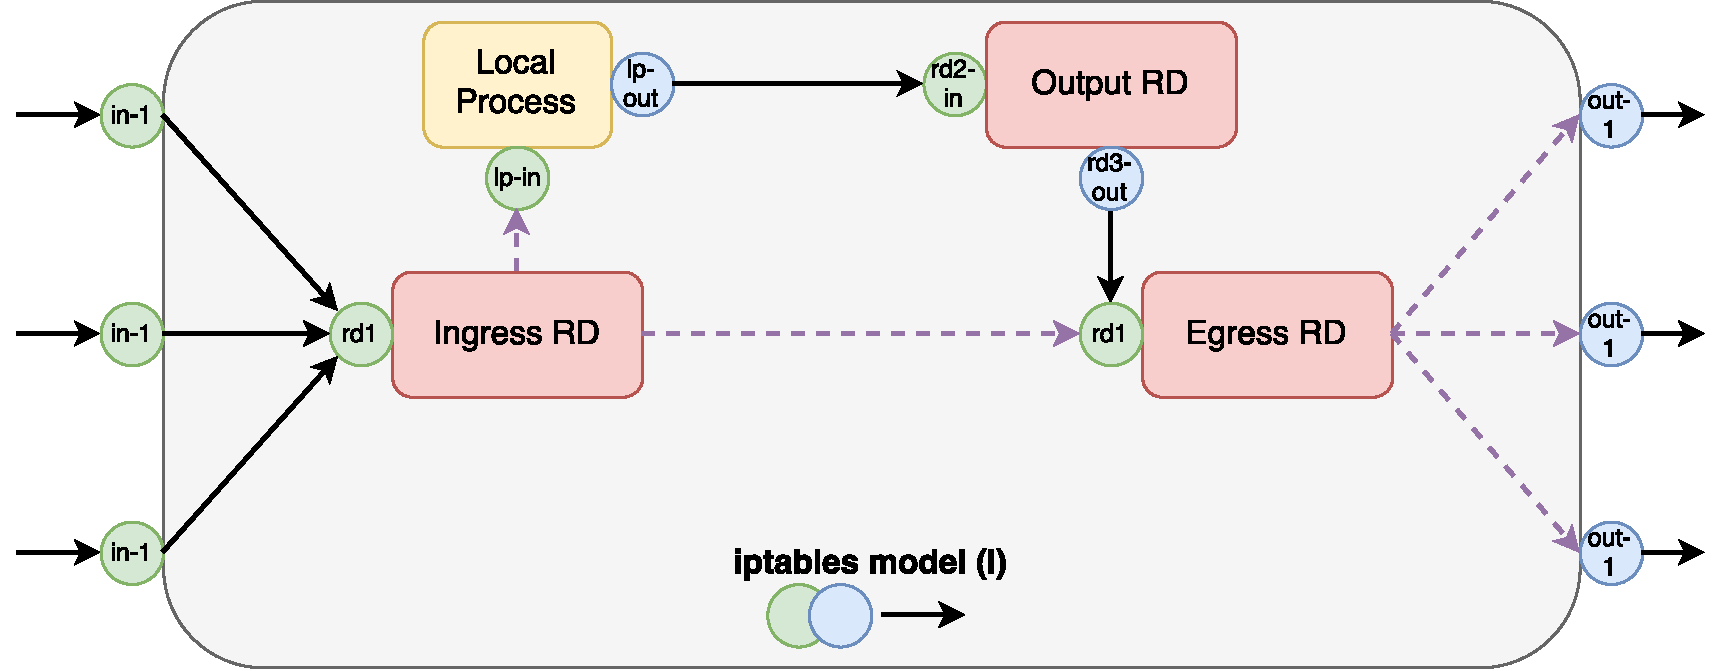
\includegraphics[scale=0.5]{src/img/iptables-1}
  \caption[iptables model (I): Separated routing decisions.]{iptables model
  (I): Separated routing decisions.\\NOTE: it is important to assign unique
  port names because there are no name scopes; implementation-wise, this is
  achieved by prefixing the \emph{role} of the port (e.g.  \emph{in},
  \emph{out}) by the unique name of the \emph{virtual device} it belongs to.}
  \label{fig:iptables-1}
\end{figure}

\todo{Give some overview of where we are currently standing and how we plan to
proceed. then.. proceed; start from router, augment it; make clear what virtual
devices are (we used this term before blabla); reiterate the encapsulation
idea}
\todo{once we show the first prototype, take some time to discuss the design:
parsing, validation, code generation, their importance, how they play together,
the fact that the table/chain/rule parsing as well as the "target" (the links
as defined in that figure, etc) are always the same, but we need to consider
the extensions-based design, etc. Mention that more details about the actual
implementation are given in section implementation}.
\todo{finish by saying that our model in figure XX hides some quite involved
logic caused by the support for user-specified chains and others, which are
discussed next..}
\todo{also show a pseudocode of the most important one, the traversal of a
chain of rules}

\subsection{User-defined chains}
\todo{explain WHY they complicate the simple model in the previous section.
explain that our final model reflects their exact semantics}
\todo{what is an Iptables Virtual Device (IVD); what is a Chain IVD; cover in
detail all components of a Chain IVD: input dispatcher, contiguous IVDs, output
dispatchers}

\subsection{Network Address Translation}
\todo{start with all kinds of NAT supported? SNAT, DNAT, MASQUERADE (mention
that it is essentially SNAT, since we model data plane only), REDIRECT}
\todo{WHY we treat NAT separately? mention the fact that for each flow, NAT
tables are consulted once only, and then the applied rule is automatically
re-applied; this means that custom logic that SKIPS the table has to be added;
show how this changes the model we reached in the previous section; add the
Chain IVD Initializer components.}
\todo{besides that, reply-packets have to be reverse-NAT'ed}

\subsection{Connection tracking}
\todo{show how we introduce a new \emph{virtual device} that implements the
connection tracking logic. mention that it is currently limited, only NEW to
ESTABLISHED is handled; explain how it works, more precisely; also mention that
a great limitation is discussed in
\labelindexref{Section}{sub-sec:related-state}.}

\bigskip
\todo{conclude by saying that it finalizes the current state of our model,
which is quite involved compared to the initial one we devised at the beginning
of this section.}


\section{Implementation}\label{sec:implementation}
\todo{Could also mention the size of the project; 4k + 4k, "out of tree"
(SymNet); not really "test-driven", but more like "tested"}
\todo{this chapter shows how some of the things discussed in the previous
section are implemented;}
\todo{add implementation-detailed diagrams of the 'iptelement' hierarchy as
well as of the 'virtualdevice' hierarchy; mention composite approach, etc.}
\todo{(inspired by todo 1 above) Discuss what the interface with SymNet is. --
these parts (Instruction/:==:, etc) will be added to a separate "api" package,
to be easily accessed by other models and for better code organization.}
\todo{Before delving into the next subsections, could also mention code
structure, 3 main directories (core, extensions - one directory for each
extension -, virtdev), the driver in the root}

\subsection{Parsing}
\todo{talk about parsing, table parsing, chain parsing, ParsingContext, rule
parsing, match/target parsing, their extensions, how they are extended, etc}
\todo{for rule parsing, mention the functionality behind the 'match extension
activation', flag -m or --match}
\todo{Monadic, Parsec, functional, haskell etc}

\subsection{Validation}
\todo{WHY it is needed; say that it is analogous to semantic analysis in
compilers}
\todo{use cases: unordered chains (needed), port range validity, certain chains
in certain tables, certain rules in certain tables/chains, etc}
\todo{how it works, validate() function, validateIf variant, ValidationContext}

\subsection{Code generation}
\todo{SeflGenOptions trait, the variant for match extensions and the one for
target extensions}


\section{Extensions}
\todo{is this section still needed? maybe add some examples in the previous
sections, rather than adding another one}
\subsection{TCP and UDP}
\subsection{MARK and CONNMARK}


\section{Limitations}
\todo{We build precise models, as far as our toolset (SymNet, SEFL) permits.
However, there are certain limitations which are discussed next.}

\subsection{The local process}
\todo{say that we are not interested in modelling the local process, as a
correct, or at least close to one, model of that would be the kernel itself,
plus application specific logic.}
\todo{however, one trick we do to allow 'simulation' of traffic generated by
some applications is to expose its output port from figure XX. this permits
starting symbolic execution by injecting a symbolic packet on that port and see
what happens, etc.}

\subsection{The RELATED connection state}\label{sub-sec:related-state}
\todo{say again what its purpose should be; give an use-case}
\todo{Inherent limitation caused by the independence between different flows.}
